% Instructions to change to html version:
% Comment out:
%  minipage, multicols,columnbreak, mathbf, hrule
% Replace all: \begin{minipage}% \end{minipage} %\begin{multicols}  %\end{multicols}  %	%% \begin{framed} %\end{framed} %%\hrule
% Replace \mathbf with	\boldsymbol
% Replace $$ with \[ or \]and $ with \( or \)
% Enclose graphics in figure environments and add captions
% 			search \includegraphics
% Re-tag \df environments as sections, subsections, etc.
% Command Line Code to Create html version:
%First: pdflatex -shell-escape filename.tex                                   
%Second, for each figure: inkscape "filename-figure1.pdf" -o "filename-figure1.png"
% Third: htlatex filename.tex "ht5mjlatex.cfg, charset=utf-8" " -cunihtf -utf8"

\documentclass[10pt]{article}

%\usepackage{tikz, pgf,pgfplots,wasysym,array}
%\usepackage{wasysym,array}

\usepackage{amsmath,amssymb}

\ifdefined\HCode
  \def\pgfsysdriver{pgfsys-tex4ht-updated.def}
\fi 
%\ifdefined\HCode
%  \def\pgfsysdriver{pgfsys-dvisvgm4ht.def}
%\fi 
\usepackage{tikz}
\usetikzlibrary{calc,decorations.markings,arrows}
\usepackage{pgfplots}

\pgfplotsset{compat=1.12}
\usepackage{myexternalize}
\usetikzlibrary{calc,decorations.markings,arrows}
\usepackage{framed}
\usepackage[none]{hyphenat}

\input{../../../common/1336_header_test.tex}
\begin{document}

\everymath{\displaystyle}

\newcommand{\limn}{\lim_{n\rightarrow\infty}}
\newcommand{\liman}{\limn a_n}

\renewcommand{\myTitle}{MATH 1336: Calculus III}

\renewcommand{\mySubTitle}{Section 5.1: Sequences}
%~\hfill Name: \underline{~~~~~~~~~~~~~~~~~~~~~~~~~~~~~~~~~~~~~~~~~~~~~~~}

\lectTitle{\vspace*{-.5in}\myTitle}{\vspace*{.1in}\mySubTitle \vspace*{-.25in}}


\setlength{\columnseprule}{0.4pt}
\setlength{\columnsep}{3em}

%\hspace*{-.8in}%\begin{minipage}{1.25\textwidth}
%\begin{framed}
%\df{\textcolor{sblack}{Infinite Sequence Definition: }}
A \textbf{sequence} is an ordered list of numbers. An \textbf{infinite sequence} is a sequence that does not terminate.
\[
\left\lbrace a_1, a_2, a_3, \ldots, a_{n-1}, a_n, a_{n+1}, \ldots \right\rbrace
\]


%\hrule
\vspace*{.1in}
\section*{Convergence/Divergence of Infinite Sequences:}

%\begin{minipage}{.4\textwidth}

\begin{figure}[!h]
\centering
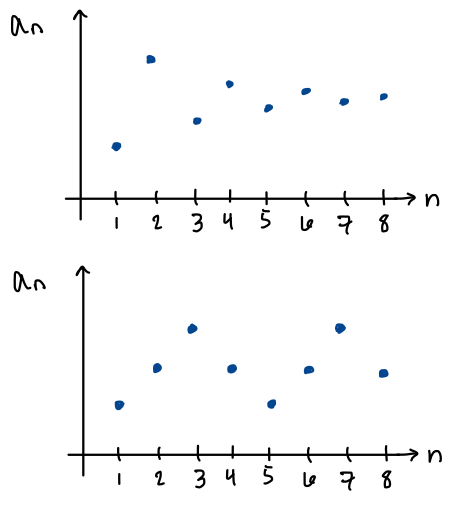
\includegraphics[width=.9\textwidth]{Ch8s1-conv-div.png}
\caption{Sequence Illustrations: First graph shows a sequence that converges, second graph shows a sequence that diverges due to oscillation.}
\end{figure}

%\end{minipage}
\hspace*{.2in}
%\begin{minipage}{.5\textwidth}
A sequence \(\lbrace a_n\rbrace\) has the limit \(L\):
\[
\lim_{n\rightarrow\infty} a_n = L,
\]
if we can make the terms \(a_n\) ``as close to L as we want'' for \(n\) sufficiently large.\\~\\
If \(\lim_{n\rightarrow\infty} a_n = L\) exists then we say that the sequence \textbf{converges} to L.\\~\\
If \(\lim_{n\rightarrow\infty} a_n \) does not exist then we say that the sequence \textbf{diverges}.\\~\\

\textbf{\(\boldsymbol{\epsilon - N}\) Limit Definition:}

The sequence \(\lbrace a_n\rbrace\) has the limit \(L\) if for every \(\epsilon>0\) there is a corresponding integer \(N\) such that\\
\[
\text{if } n > N, \textbf{ then } |a_n - L| < \epsilon.
\]
~\\

%\textit{If you want to review, you can find Limit Laws and the Squeeze Theorem in section 1.4 and L'Hopital's Rule in section 3.7.)}

%\end{minipage}
%
%%\hrule
%\vspace*{.1in}
%\df{\textcolor{sblack}{Convergence/Divergence of Infinite Sequences:}}~\\
%
%
%\textbf{Theorem 3:} If \(\lim_{x\rightarrow\infty} f(x) = L\) and \(f(n)=a_n\) when \(n\) is an integer, then \(\lim_{n\rightarrow\infty} a_n = L\).

%\end{framed}
%\end{minipage}

%\section*{Problems for Group Work/Examples:}
\vspace*{.1in}
Write out the first four terms of the sequence to build your intuition.\\ %(You may want to sketch graphs of the sequences as well.)
Then, determine the convergence or divergence of the sequences.\\ %Be sure to write out the first four terms of the sequence. 
%(You may also want to sketch graphs of the sequences as well.)\\ 
\textbf{Be sure to fully justify your conclusions using tools found on the next page.}
\vfill
\setlength{\columnseprule}{0pt}
\begin{enumerate}

%\begin{multicols}{2}

\item \(\qquad a_n = \frac{n}{1+n^2}\) \vspace*{.25in}

\item \(\qquad b_n = \frac{\ln(1+2e^n)}{n}\) \vspace*{.25in}

\item \(\qquad c_n = \sin(n\pi)\)\vspace*{.25in}

\item \(\qquad d_n = \frac{1+n\cos(2\pi n)}{n}\)\vspace*{.25in}

\item \(\qquad a_n = \frac{e^n}{3^n}\)\vspace*{.25in}

\item \(\qquad b_n =(-1)^n \sqrt{n}\) \vspace*{.25in}

\item \(\qquad c_n =(-1)^n \frac{1}{\sqrt{n}}\) \vspace*{.25in}

\item \(\qquad d_n =(-1)^{2n+1} \) \vspace*{.25in}

%\end{multicols}
\vfill

\item \textbf{Challenge Problem:} Note that \(n\) factorial is defined as \(n! = 1\cdot 2 \cdot 3 \cdot \ldots \cdot (n-1) \cdot n \)\\
 \(\qquad a_n =\frac{(-3)^n}{n!} \) 

\vfill
\end{enumerate}

\pagebreak

\section*{Tools for Finding Limits of Sequences:}\label{limitlaws}

%\hspace*{-.8in}\begin{minipage}{1.25\textwidth}
%\begin{framed}
\subsection*{The following limit laws can be used without a formal citation:}
%\textit{The following limit laws and theorems can be used without a formal citation.}\\
\textbf{Limit Laws for Sequences:}\\
Given 
\[
\liman = L_1, \qquad \limn b_n = L_2, \qquad c:\text{ some finite constant}
\]
then
%\begin{multicols}{2}

\[ \limn ( a_n \pm b_n) = L_1 \pm L_2\]

\[ \limn c\ a_n = c\ L_1\]

\[ \limn (a_n b_n) = L_1 L_2\]

\[ \limn c = c\]



\[ \limn \frac{a_n}{b_n} = \frac{L_1}{L_2} \quad \text{if } L_2 \neq 0 \text{ and none of the } b_n = 0\]

\[ \limn \left(a_n\right)^p = \left(L_1\right)^p \quad \text{ if } p>0 \text{ and } a_n > 0\]
~\\

%\textbf{Theorem 6:} 
If \(\limn | a_n | = 0\) then \(\liman = 0\).

%\end{multicols}

%\hrule
\vspace*{.1in}

\subsection*{The following theorems must be formally cited when used:}



%\begin{minipage}{.5\textwidth}

\textbf{Theorem 5.4: Squeeze Theorem:}\\

If \(a_n \leq b_n \leq c_n\) for \(n \geq n_0\) and 
\[
\limn a_n = \limn c_n = L,
\]
then \(\limn b_n = L.\)
~\\

%\end{minipage}
\hspace*{.2in}
%\begin{minipage}{.4\textwidth}


\begin{figure}[!h]
\centering
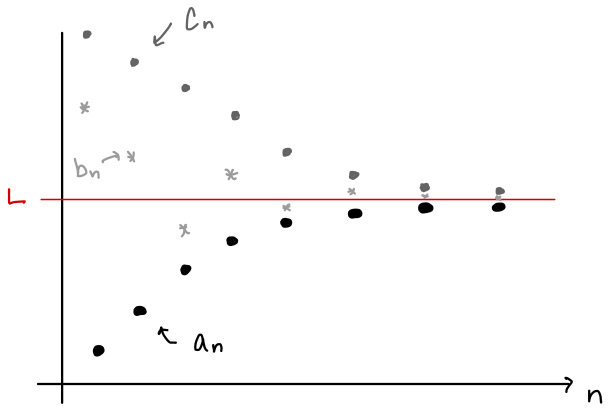
\includegraphics[height=1in]{Ch8s1-squeeze.png}
 \caption{Figure illustrates the Squeeze Theorem for sequences.}

\end{figure}

%\end{minipage}


\textbf{Theorem 5.3: Continuity \& Convergence Theorem:}\\
If \( \liman = L\) and \(f\) is continuous at \(L\), then \( \limn f(a_n) = f(L)\).\\




\textbf{Theorem 5.1:} If \(\lim_{x\rightarrow\infty} f(x) = L\) and \(f(n)=a_n\) when \(n\) is an integer, then \(\lim_{n\rightarrow\infty} a_n = L\).\\
\textit{(In the previous textbook for this class, this was ``Theorem 3,'' which may still appear in my notes/solutions as we transition to the new textbook.)}\\


%\hrule
\vspace*{.1in}
\subsection*{If you want to use L'Hopital's Rule:}
First switch to a function, \(f\),  of the \textit{continuous} variable \(x\), such that \(f(n) = a_n\) when \(n\) is an integer.\\
Then use L'Hopital's Rule to find the limit of the \textit{continuous} function \(f(x)\) as \(x\rightarrow \infty\).\\
Finally, cite Theorem 5.1.



%\end{framed}
%%\end{minipage}

%
%\pagebreak
%
%\includegraphics[height=\textheight]{Ch8s1-limit-laws}

\end{document}
